%!TEX root = main.tex

\begin{figure*}[!t]
\centering
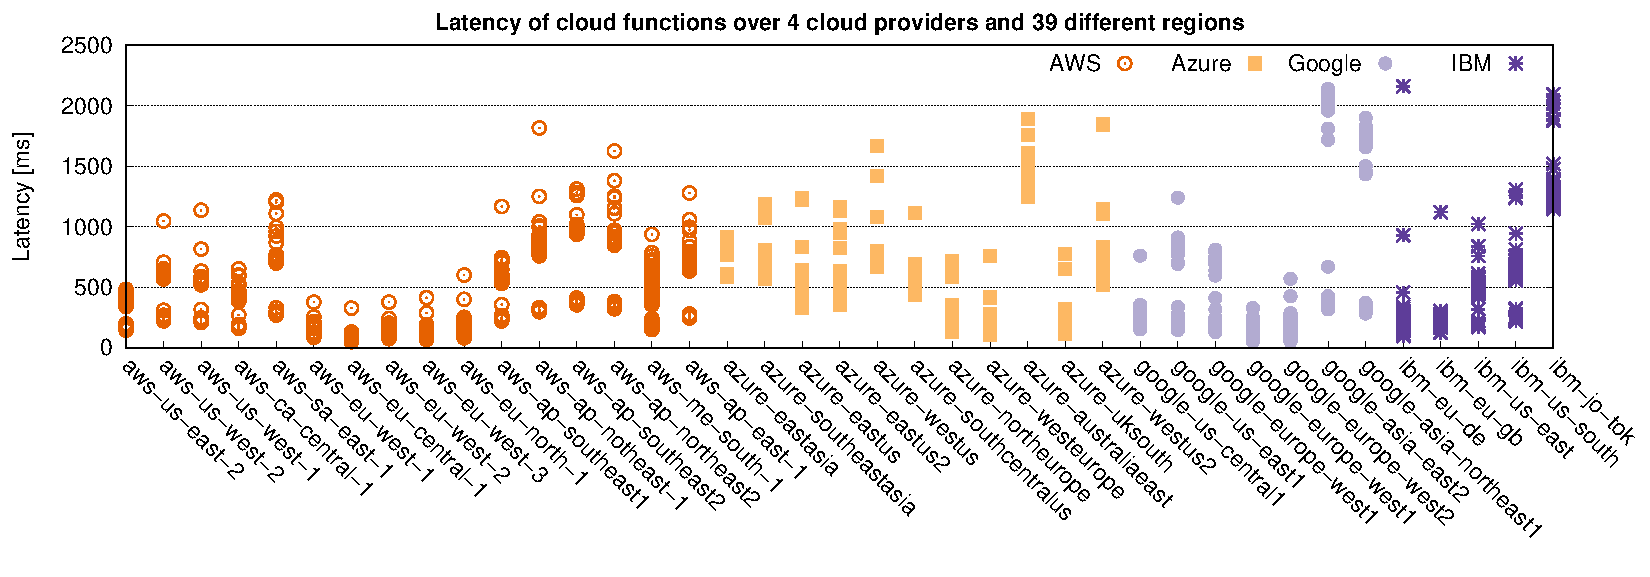
\includegraphics[width=1.0\textwidth]{bilder/latency/latency}
\caption{Latency test scatter plot. Since \texttt{azure-west-us} had issues with Node.js, we resort to \texttt{.NET} for that zone.}
\label{fig:latency_plot}
\end{figure*}

\section{Evaluation}
\label{sec:evaluation}

We present in this section the results of our evaluation using \sys of the different FaaS providers supported by our current implementation.
% Rather than benchmarking the internal components of \sys, this section presents the typical evaluation results that be easily produced using \sys.
We carried out these tests over a period of three weeks (Jan. 13--Feb. 4, 2020).
These experiments specifically aim at answering the following questions: 
\emph{(1)} what is the most effective programming language to use for serverless applications;
\emph{(2)} what is the most convenient provider; and
\emph{(3)} which provider yields the most predictable results.

%chapter results of performed tests will be presented and explained, an example for a pricing calculation will be given, the services among the cloud providers will be compared and some general advantages and disadvantages about serverless computing will be specified derived from these results.
%
%In this thesis, four different tests have been performed. Each one will be discussed in detail and results will be presented in the following subsections.

\subsection{Call Latency}
\vs{clarify these are valid for the region from where we computed those}
We begin by measuring the latency (round-trip) for all cloud providers and corresponding regions, using the \texttt{faas-netlatency} benchmark.
%This test differs from a normal ping, that effectively a cloud function is executed instead of just returning a message on a more abstract level. 
Unless specified otherwise, we deploy Node.js using 128\,\gls{MB}.
We note that AWS functions run under a custom kernel 4.14.138-99.102.amzn2.x86\_64;\footnote{\url{https://docs.aws.amazon.com/lambda/latest/dg/lambda-runtimes.html}} 
whole host configurations are not disclosed for Azure, Google or IBM deployments.
%\mais{Azure, Google and IBM do not mention anything about the OS. Unfortunately that did not come to my mind when testing it. I can try to find things out by executing commands like 'uname -a'. Please let me know if I shall do that.}.   
%The test was performed in Node.js with 128\gls{MB} of memory (Azure 1.5\gls{GB}) with the latency test described in section \ref{subsec:latency}. 
A request is sent every 5 seconds to each cloud and region, up to 100 samples per function.
\autoref{fig:latency_plot} reports our results across 39 different configurations. 
%This test was carried out from Bern, Switzerland.
%\begin{remarks}
%\text{ }
%\begin{itemize}
%    \item For Azure, this test was only done with Linux as underlying OS. The OS should not matter in regards to latency.
%    \item The \textit{westus} region of Azure had problems deploying it in Node.js and therefore .NET was used. Following error was produced: \texttt{The scale operation is not allowed for this subscription in this region. Try selecting different region or scale option.}\\
%    Also trying to create the function in the Azure portal failed and an error was indicated but the error message could not be viewed.
%    \item On Azure region \textit{australiaeast} the function could not be deployed, although no error was risen. Therefore it was deployed on Windows instead of Linux.
%\end{itemize}
%\end{remarks}
%The graphic \ref{fig:latency_plot} shows a scatter plot with the results of the test.
%\vs{MAISSEN: here we need a short discussion on the results. Something like the following, can you complete ? I'll check afterwards}. %\mais{OK?}
%We observe the following.
The average latency over all clouds and regions is 538\,ms.
We achieve the fasted result on AWS Lambda (\texttt{eu-central-1}) at 80\,ms, and the slowest toward Google (\texttt{asia-east2}) at 1,770\,ms. 
Overall, the best performing cloud provider is Amazon, with slightly lower latency for the same geographical locations of other providers. \mais{This benchmark was performed from Bern, Switzerland and results will vary depending on the location of execution.}

%For more detailed results see table \ref{tab:latency}. 
%The raw result file, R script and plot image are also on \href{https://github.com/Bschitter/benchmark-suite-serverless-computing/tree/master/results/1-latency}{GitHub}.

\subsection{Cold Start}
\label{sec:coldstart}
\vs{clarify experimental methodology, provide further details if possible}
%This test measured the cold start latency. 
A cold start happens when a function takes longer than usual to execute. 
Most of the time, this occurs when the invocation is scheduled right after the completion of its deployment, or when the function has not been used in a while, \eg, after 10 minutes without invocations.
%However, we observed longer timings, for instance on Google, with up to 10 hours before de-allocating the instance. \mais{I don't understand the previous sentence.}
Specifically, there are several steps to perform before a function can execute: allocate a server, set up a worker with the associated code, packages and extensions, load the function in memory, and finally run it.
These steps contribute clearly to the cold start effect that we observe in our results.
When the function is \emph{warm}, it is ready in memory and can immediately serve requests.
A function can also be de-allocated (\ie, garbage-collected) when a new instance needs to be provisioned for scaling purposes. 
When this happens and an invocation is scheduled for the just garbage-collected function, the cold start effect is clearly measurable with degrading effects on the measured latency.
%\vs{MAISSEN: can't understand this sentence, can you rephrase?} \mais{In order for the cloud provider to prepare the VM instance and deploy the user function code on it, some time can pass.}
\autoref{fig:azure_coldstart} shows the execution workflow for a cold start on Azure, as opposed to the warm case. 
Similar workflows (and effects on latency) exist on the other cloud providers.\footnote{Refer for instance to \url{https://cloud.google.com/functions/docs/bestpractices/tips} for information and best practices from Google.}
%\vs{MAISSEN: do you have the same results for the other providers? eg, why only Azure?} \mais{This is just exemplary done for Azure. Should be very similar on other clouds. see \url{https://cloud.google.com/functions/docs/bestpractices/tips} , little doc of providers because a 'disadvantage' of serverless}

\begin{figure}[!b]
\centering
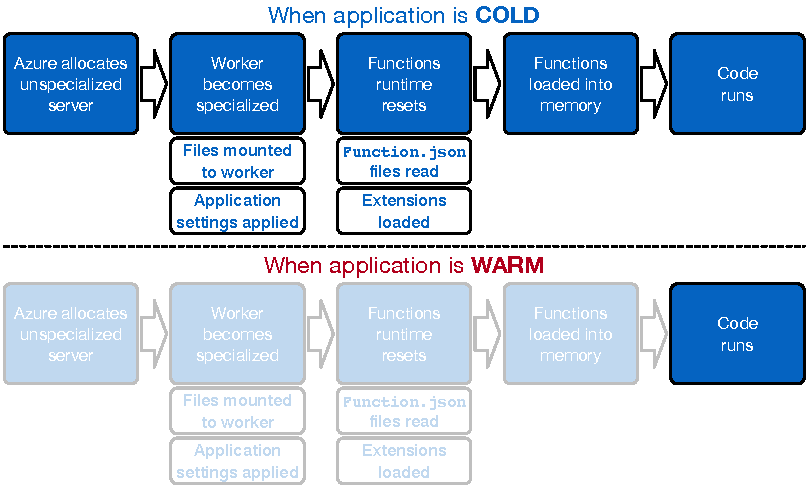
\includegraphics[scale=0.6]{bilder/cold-warm}
\caption{Workflow for cold and warm start on Azure~\cite{AzureColdStart}.}
\label{fig:azure_coldstart}
\end{figure}

\begin{figure}[!t]
\centering
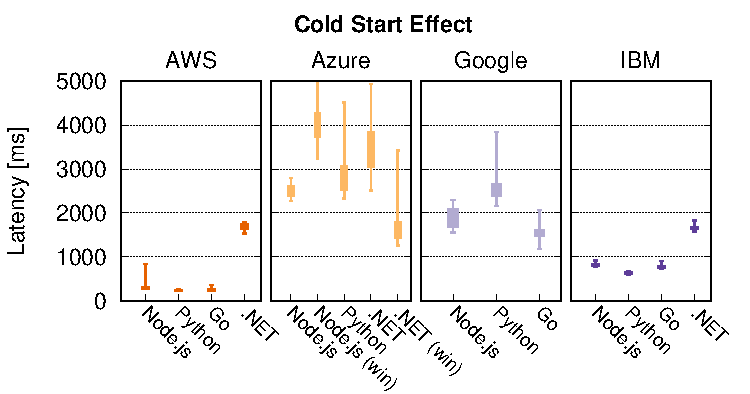
\includegraphics[scale=0.7]{bilder/cold_start/coldstart_whisker}
\caption{Cold start latency.}
\label{fig:coldstart_plot}
\end{figure}

Our results are averaged over ten executions for each configuration runtime/cloud. 
Functions are executed using 512\,\gls{MB} of memory and without external packages, to reduce the baseline footprint and the corresponding loading time to the bare minimum.
%The cold start latency has been tested ten times for each runtime on each cloud.
%Memory size was defined with 512 \gls{MB} and no packages were loaded into the function. 
We executed these tests on the following regions: \texttt{eu-central-1} for AWS, \texttt{west-europe} for Azure,  \texttt{europe-west1} for Google and \texttt{eu-de} for IBM. 
Note however that the chosen region has no impact on the cold start latency. 
We compute the cold start latency as the total request time minus the normal average latency. \mais{Cold starts were deteced with the help of instance IDs on AWS and IBM. On Azure and Google online metrics of running instances were taken into account to verify cold starts. The challenge of cold start detection lead to a manual test execution and data manipulation.}

\begin{figure}[!b]
\centering
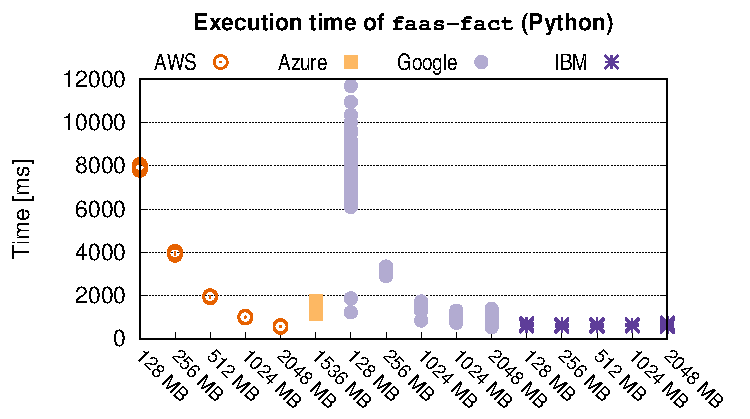
\includegraphics[scale=0.7]{bilder/general_python/cpufact.pdf}
\caption{Execution time of \texttt{faas-fact} in Python.}
\label{fig:general_python_plot}
\end{figure}

\begin{figure}[!b]
\centering
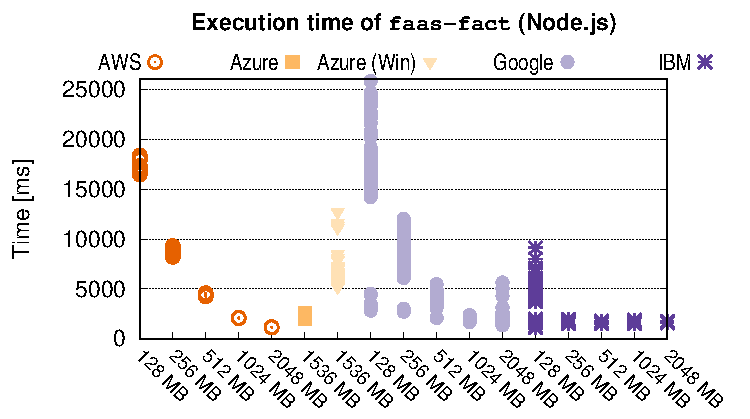
\includegraphics[scale=0.7]{bilder/general_node/cpufact.pdf}
\caption{Execution time of \texttt{faas-fact} in Node.js.}
\label{fig:general_node_plot}
\end{figure}

\autoref{fig:coldstart_plot} summarizes our results using a box-and-whiskers plot.
It stands out that \gls{AWS} is overall the fastest, with an average cold start latency of only 335\,ms for Node.js, Python and Go. 
Results with .NET are worse, with latencies up to 1,739\,ms, likely due to the nature of the runtime and the compilation of C\#. 
On Azure, cold start latency is strictly more than 2 seconds and up to 5 seconds, with the exception of the combination .NET on Windows, which averages at 1,917\,ms. 
IBM compares similarly to \gls{AWS}.
Finally, Google Cloud consistently yields higher cold start latencies, in the 2-3 seconds range. 
\gls{IBM} exhibits a performs similarly to \gls{AWS} across the spectrum of supported languages, although the cold start latency is around 600\,ms higher for Node.js, Python and Go but similar for .NET.

%\vs{MAISSEN: what is this 'reclying' you refer to ? can you clarify?} \mais{Recycling meaning in this context deallocating a VM instance of the user and make it available to all users in the cloud's total pool}
On \gls{AWS} and \gls{IBM}, it took usually around 10 minutes of no activity for the computing instance to be recycled by the provider and re-inserted into the pool of available ones, and up to 20 minutes on Azure.
On Google, this time varied from 10 minutes up to 10 hours. %\mais{I said to you 12 hours as mentioned previously in this section. I meant also 10. I corrected this, you can remove this comment.}

\subsection{CPU-bound Benchmarks}
\label{sec:general_test}

%This test was performed to analyze the functions under normal circumstances, meaning that there is not much load respectively that the load can be handled well by the cloud provider. The objective is to compare the achieved performance of the clouds regarding execution speed and the thereby implicated costs. 
This benchmark evaluates how CPU-bound workloads behave across the different cloud providers.
% evaluation the \gls{CPU} factors test (see section \ref{sec:factors_test}) was executed. 
A function (\texttt{faas-fact}) is invoked every five seconds, using as parameter a large integer triggering a sufficiently challenging computation. 
We collect 100 results for every configuration (runtime, memory, cloud provider).
%The function was invoked every five seconds until a sample size of $n=100$ was reached. 
%This for each \gls{MB} configuration, each runtime and each cloud. 
%s input parameter $26'888'346'474'443$ was selected since with this number the function finished ahead of the timeout for low configurations and simultaneously was not too quickly finished for high configurations. 
We report these results for all cloud configurations and languages: Python (\autoref{fig:general_python_plot}), Node.js (\autoref{fig:general_node_plot}), Go (\autoref{fig:general_go_plot}) and .NET (\autoref{fig:general_dotnet_plot}).
%Figure~\ref{fig:general_python_plot} depicts our result for Python
%\vs{If we have time, we could include the same plots for the other languages. MAISSEN: could you give it a try, using the Python example as template to produce them? }

\begin{figure}[!b]
\centering
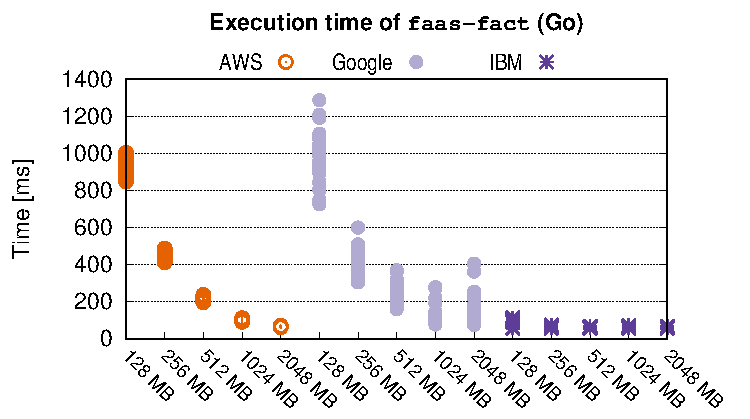
\includegraphics[scale=0.7]{bilder/general_go/cpufact.pdf}
\caption{Execution time of \texttt{faas-fact} in Go.}
\label{fig:general_go_plot}
\end{figure}

\begin{figure}[!b]
\centering
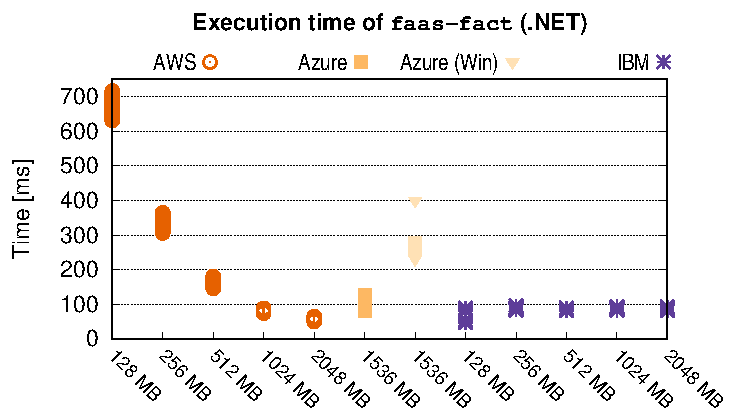
\includegraphics[scale=0.7]{bilder/general_dotnet/cpufact.pdf}
\caption{Execution time of the \texttt{faas-fact} in .NET.}
\label{fig:general_dotnet_plot}
\end{figure}

We note a few interesting facts.
On \gls{AWS} Lambda, the standard deviation is low, with a minimum value of 50\,ms using .NET and  2,048\,MB of memory, with very consistent execution times across all the different configurations. 
As expected, every doubling of the allocated memory results in halving the execution time, \ie, performance scales linearly with allocated memory~\cite{AWSLambdaConfig}. 

\begin{figure*}[!t]
\centering
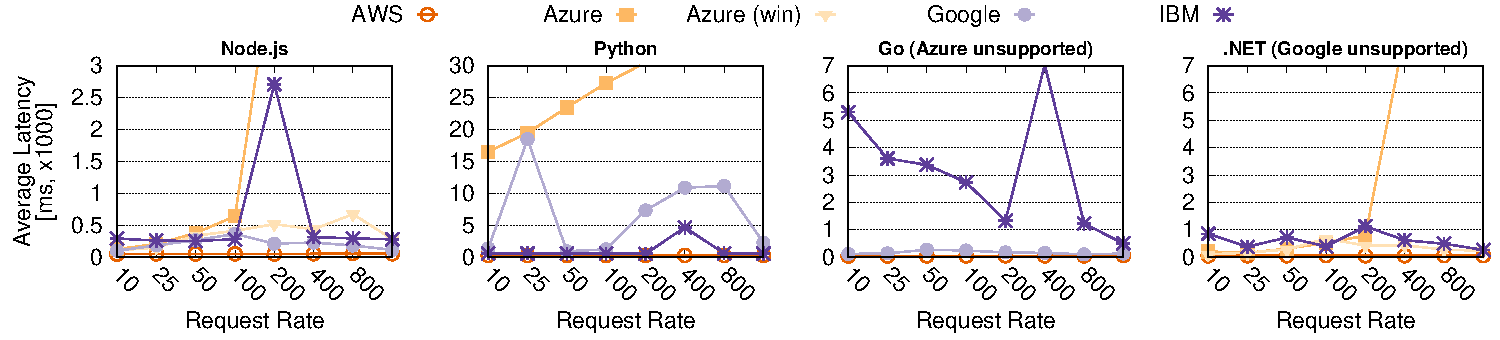
\includegraphics[scale=0.7]{bilder/loadtest_average_latency/tputlat_combined}
\caption{Throughput/latency benchmark using \texttt{wrk2}~\cite{wrk2} and \sys's  \texttt{faas-matrix-mult} stress function.}
%\mais{Something's wrong. Did you intentially not plot Azure Windows for Node.js and .NET? Further, the .NET plot is wrong: AWS not plotted, Azure (Linux) has the color of AWS}}
\label{fig:load_test_latency_all}
\end{figure*}

Azure's memory configuration of 1,536\,\gls{MB} suggests its performance to be in the 1,024-2,048\,\gls{MB} range.
Surprisingly, it is slower than 1,024\,\gls{MB} instances of the other clouds.  
Google Cloud Platform performs similarly to \gls{AWS}, although more scattered for 128\,\gls{MB} of memory. 
Google achieves better results than \gls{AWS} for several memory configurations (128, 256, 512 and 1,024\,\gls{MB}). % but not for 2048 \gls{MB}. For the first three times doubling the memory leads to halved execution time. 
Note however that the performance scaling behaves differently on the Google platform~\cite{GoogleFunctionsPricing}.
%But not entirely for the next two steps since Google does not scale \gls{CPU} completely linear to allocated memory \cite{GoogleFunctionsPricing}. 
The results we gathered on the \gls{IBM} platform suggests that memory allocation does not correlate with \gls{CPU} allocation in any way, with five different configurations performing very closely. 
This is remarkable since the pricing model of \gls{IBM} only accounts for the GB-seconds used. 
%\vs{MAISSEN: Is this true for all the languages? These resuls are only for Phython. Do you have the same tests for all the other languges? This means that a user could deploy his application always with the smallest memory option possible and would thereby get the same performance for the smaller price.} \mais{Yes this is true for all languages, see {https://github.com/Bschitter/benchmark-suite-serverless-computing/blob/master/results/3-general} files with name scatterplot\_general\_<RUNTIME>.png}
%The results and plots for this and the three other runtimes can be found on \href{https://github.com/Bschitter/benchmark-suite-serverless-computing/tree/master/results/3-general}{GitHub}.

\subsection{Throughput/Latency}
\label{sec:loadtest}

To understand the saturation point of the deployed services, we rely on \texttt{wrk2}~\cite{wrk2}, a constant throughput/exact latency HTTP-based benchmarking tool.
We configure this benchmark to issue function call invocations at increasingly high rates, from 10 up to 1,000 requests per second.
For each of the configurations, \texttt{wrk2} reports the average latency to handle the requests (\ie, the functions).
Between each configuration, the benchmark waits for sufficient time to process any request still possibly enqueued.
\autoref{fig:load_test_latency_all} shows our results for the \texttt{faas-matrix-mult} function and the 4 different programming languages under test.
%The load test is designed to benchmark the serverless functions up to 1000 requests per second. 
%This is carried out with the \gls{HTTP} benchmark tool \textit{wrk2} (see \cite{wrk2}). A function is first called with 10 requests per second for the duration of 1 minute. 
%Subsequently with 25, 50, 100, 200, 400, 800 and finally 1000 requests per second each time for one minute. 
%In between is a short break of 10 seconds to allow the function to process requests that are still queued. As test, the matrix function with a parameter of 100 is used. With this setup the matrix function should have an average execution time of about 100ms for Node.js, Go and .NET and around 250ms for Python. The graphic \ref{fig:load_test_latency_all} displays the average latency results grouped by runtime.
%The results are now discussed step by step. 

We observe that \gls{AWS} achieves stable response latencies for all the tested workloads. 
%This is very remarkable and a very good result and can be probably traced back to the low cold start latency and the good and consistent performance presented in section \ref{sec:general_test}.\\
Azure, on the other hand, shows more surprising results.
Whereas it can tolerate high loads on Windows OS, it performs very inconsistently on Linux.
The response latency grows almost linearly with the total requests per second injected and quickly saturates. 
That is a strong indication that none (or too few) new instances were allocated to handle the load. 
We investigated this behaviour further through the Azure portal Live Metrics Stream (not shown). 
When reaching 1,000 requests per second, only a total of 12 instances were deployed to serve .NET functions. % have been deployed (see figure \ref{fig:live_metrics_stream}). 
Additionally, only 500 requests per second were actually served, leaving a large percentage of requests in the waiting queue.
%\begin{remark}
%In the screenshot the request duration differs from the wrk2 results since that is most likely only considering execution time without queuing time.
%\end{remark}

%\begin{figure}[htp]
%\centering
%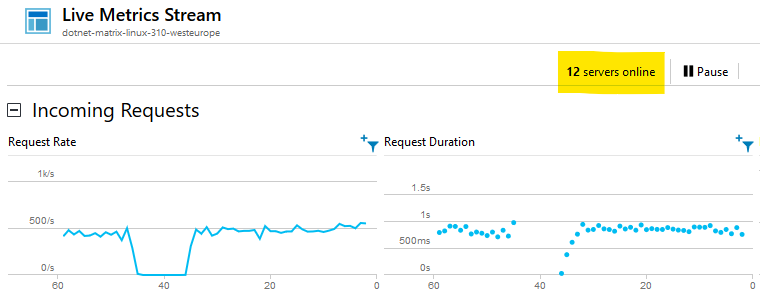
\includegraphics[scale=0.3]{bilder/Azure_Dotnet_1000.png}
%\caption[Azure Linux .NET Live Metrics Stream during 1000 RPS]{Azure Linux .NET Live Metrics Stream during 1000 RPS\\Source: screenshot Azure portal}
%\label{fig:live_metrics_stream}
%\end{figure}

\renewcommand{\arraystretch}{1.2}
\begin{table}[!t]
\setlength{\tabcolsep}{3pt}
\scriptsize
\centering
\caption{Latency: goal/target, results in the long-tail (below 90\% of the target requests/sec).}
\rowcolors{1}{gray!10}{gray!0}
\begin{tabular}{l|l|r|r|r} 
\rowcolor{gray!45}
\textbf{Cloud} & \textbf{Runtime} & \textbf{Req/s (goal)} & \textbf{Req/s (actual)} & \textbf{Req/s (\%)} \\ \hline
%\rowcolor{gray!25}
Azure & Node.js & 200 & 179 & 89.50\% \\ 
Azure & Node.js & 400 & 227 & 56.75\% \\ 
Azure & Node.js & 800 & 278 & 34.75\% \\ 
Azure & Node.js & 1000 & 327 & 32.70\% \\
Azure & Python & 10 & 6 & 60.00\% \\  
Azure & Python & 25 & 12 & 48.00\% \\ 
Azure & Python & 50 & 18 & 36.00\% \\ 
Azure & Python & 100 & 25 & 25.00\% \\ 
Azure & Python & 200 & 30 & 15.00\% \\ 
Azure & Python & 400 & 15 & 3.75\% \\ 
Azure & Python & 800 & 14 & 1.75\% \\ 
Azure & Python & 1000 & 15 & 1.50\% \\
Azure & .NET & 400 & 324  & 81.00\% \\
Azure & .NET & 800 & 407 & 50.88\% \\ 
Azure & .NET & 1000 & 512 & 51.20\% \\ 
Google & Python & 25 & 12 & 48.00\% \\ 
Google & Python & 200 & 168 & 84.00\% \\ 
Google & Python & 400 & 297 & 74.25\% \\ 
Google & Python & 800 & 575 & 71.88\% \\ 
IBM & Go & 25 &  21 & 84.00\% \\ \hline
\end{tabular}
\label{table:rps}
\vspace{-15pt}
\end{table}

For Node.js and .NET, response latencies spike up to 24\,s and 18\,s, respectively. % and are not plotted in the graph for illustration purposes. 
Using Python, Azure managed to handle up to 200 requests per second, beyond which none of the requests could be served correctly.
Google can manage the load generally well, although latency increases slightly for Node.js and Go. 
However, Python functions deployed Google suffer from poor performance, in particular at higher request rates. 
Results suggest poor capacity in adapting quickly to flash-crowd requests, with the average request duration growing from 1,356 to 18,448\,ms when increasing the rate from 10 to 25 requests per second. 
%After that, this phenomena happens again but less drastically. 
%Since functions take on average a longer time to execute in Python, it seems and Google can scale longer running functions less good. %Overall the performance is good. 
We investigate further (\autoref{fig:google_graph_go}) by analyzing the scaling behaviour for instances running Google Functions.
The plot shows the number of instances allocated during the load test on Google, suggesting indeed that the auto-scalability features provided by the infrastructure might lead to poor results as requests start saturating the deployed instances.
%\vs{this was for Go}

\begin{figure}[!t]
\centering
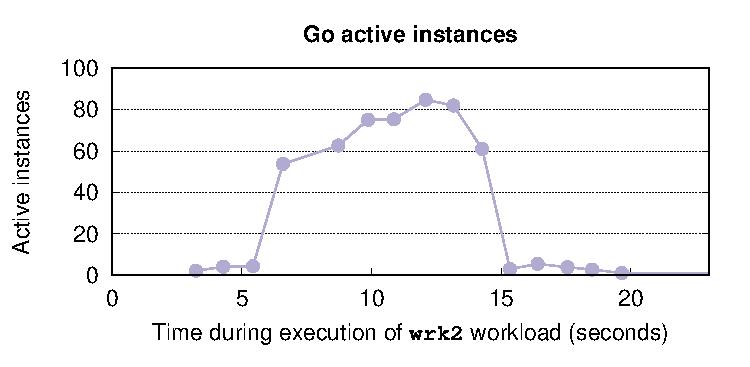
\includegraphics[scale=0.7]{bilder/go_instances/go_instances}
\caption{Google Go: number of active compute instances during the wrk2 load test.}
\label{fig:google_graph_go}
\end{figure}

%Finally, we discuss the results obtained using \gls{IBM} Cloud Functions.
%Lastly, the result of \gls{IBM} will be discussed. 
%Those outcomes differ from the others relatively much. 
On \gls{IBM} Cloud Functions, Node.js performs particularly poorly when compared to the other providers, while Python functions perform on par with \gls{AWS}.
Go functions achieve far worse than for other providers, contrasting with the cold start results that suggested similar behaviour. 
Further investigation is needed as part of future work to understand the reasons of this behaviour.
%On Node.js and .NET it can roughly keep up to the competition but operates a little slower and on Node.js it has a striking outlier. 
%The Python function on IBM nearly performs as well as on \gls{AWS}, but the same cannot be said about Go. 
%The Go runtime performed much slower in the load test as with the competitors, although as seen in the cold start test in section \ref{sec:coldstart} it has a similar cold start latency as Node.js and Python and as shown in the appendix table \ref{tab:general} it performs generally well on Go. 
%Thus this bad performance cannot be derived from this or other tests and it is possible that IBMs auto scaling mechanism does not work well for Go. 
%Of the amount of instances deployed, IBM delivers no statistics.
%\vs{MAISSEN: can you confirm I understood correctly the results in table 3?} \mais{Yes I think so, but bad wording for the last sentence. ->  In particular, we only report the cases which achieved 90\% and below of the target throughput (right-most column).}
\autoref{table:rps} reports for which cases the target throughput set by \texttt{wrk2} could not be reached within a 10\% margin, \ie, cases achieving at most 90\% of the target throughput (right-most column).
%So far, the latency has been examined and now the actual throughput will be explained. Most of the cloud providers and runtimes could handle the load and only had an irrelevant smaller throughput than tested against. Therefore only significant impacts in throughput will be presented, meaning that the throughput was less than 90\% of the tested one. The subsequent table \ref{table:rps} shows where throughput was below 90\%.
%In addition, there are detailed result plots (figure \ref{fig:loadtest_percentile_node} - \ref{fig:loadtest_percentile_dotnet}) and tables (table \ref{table:aws_load_test} - \ref{table:ibm_load_test}) in the appendix.

%\begin{table}[!t]
%\centering
%\scriptsize
%\setlength{\tabcolsep}{3pt}
%\caption[Pricing example regarding test results]{Pricing example regarding test results}
%\begin{tabular}{l|c|c|c|c|c|c} 
%     &   \textbf{Rounded time}  & \textbf{Invocation} & \textbf{GB-Seconds} & \textbf{GHz-Seconds} & \textbf{Network} & \textbf{Total} \\ \hline
%AWS  128MB      & 8000~ms &  2.00\$  &  166.67\$     &  -        & 3.43\$ & 172.10\$ \\ \hline
%AWS  256MB      & 4000~ms &  2.00\$  &  166.67\$     &  -        & 3.43\$ & 172.10\$ \\ \hline
%AWS  512MB      & 2000~ms &  2.00\$  &  166.67\$     &  -        & 3.43\$ & 172.10\$ \\ \hline
%AWS 1024MB      & 1000~ms &  2.00\$  &  166.67\$     &  -        & 3.43\$ & 172.10\$ \\ \hline
%AWS 2048MB      &  600~ms &  2.00\$  &  200.00\$     &  -        & 3.43\$ & 205.43\$ \\ \hline
%Azure 128MB     & 1267~ms &  2.00\$  &   25.34\$     &  -        & 3.32\$ &  30.66\$ \\ \hline
%Google  128MB   & 7700~ms &  4.00\$  &   24.06\$     &  154.00\$ & 4.58\$ & 186.64\$ \\ \hline
%Google  256MB   & 3200~ms &  4.00\$  &   20.00\$     &  128.00\$ & 4.58\$ & 156.58\$ \\ \hline
%Google  512MB   & 1600~ms &  4.00\$  &   20.00\$     &  128.00\$ & 4.58\$ & 156.58\$ \\ \hline
%Google 1024MB   &  900~ms &  4.00\$  &   22.50\$     &  126.00\$ & 4.58\$ & 157.08\$ \\ \hline
%Google 2048MB   &  800~ms &  4.00\$  &   40.00\$     &  192.00\$ & 4.58\$ & 240.58\$ \\ \hline
%IBM  128MB      &  700~ms &  -       &   14.88\$     &  -        & -      &  14.88\$ \\ \hline
%IBM  256MB      &  600~ms &  -       &   25.50\$     &  -        & -      &  25.50\$ \\ \hline
%IBM  512MB      &  600~ms &  -       &   51.00\$     &  -        & -      &  51.00\$ \\ \hline
%IBM 1024MB      &  600~ms &  -       &  102.00\$     &  -        & -      &  102.00\$ \\ \hline
%IBM 2048MB      &  700~ms &  -       &  238.00\$     &  -        & -      &  238.00\$ \\ \hline
%\end{tabular}
%\label{table:example2}
%\end{table}

\begin{table}[!t]
    \caption{Pricing calculation: cost of the CPU-bound benchmarks computed by \sys according to the pricing models of each cloud. \mais{Execution times are rounded up to the next 100\,ms for AWS, Google and IBM \cite{AWSPricing, GoogleFunctionsPricing, IBMPricing}}.
    \label{table:example2}}
    \setlength{\tabcolsep}{3pt}
  \scriptsize
  \center
  \rowcolors{1}{gray!10}{gray!0}
  \begin{tabular}{r|r|r|r|r|r|r}
  \rowcolor{gray!45}
  \textbf{Memory} & \textbf{Exec. time}  & \textbf{Invocation} & \textbf{GB/sec} & \textbf{GHz/sec} & \textbf{BW} & \textbf{Total} \\
    \hline
  \rowcolor{gray!25}
    AWS  & & & & & &\\
    128\,MB & 8000\,ms &  2.00\$  &  166.67\$  &  --- & 3.43\$ & 172.10\$ \\
    256\,MB & 4000\,ms &  2.00\$  &  166.67\$  &  --- & 3.43\$ & 172.10\$ \\
    512\,MB & 2000\,ms &  2.00\$  &  166.67\$  &  --- & 3.43\$ & 172.10\$ \\
	1\,GB   & 1000\,ms &  2.00\$  &  166.67\$  &  --- & 3.43\$ & 172.10\$ \\
	2\,GB &  600\,ms &  2.00\$  &  200.00\$  &  --- & 3.43\$ & 205.43\$ \\
    \hline
  \rowcolor{gray!25}
    Azure  & & & & & &\\
    128\,MB & 1267\,ms &  2.00\$  &   25.34\$     &  ---        & 3.32\$ &  30.66\$ \\
    \hline
  \rowcolor{gray!25}
    Google  & & & & & &\\
    128\,MB & 7700\,ms &  4.00\$  &   24.06\$     &  154.00\$ & 4.58\$ & 186.64\$ \\
    256\,MB & 3200\,ms &  4.00\$  &   20.00\$     &  128.00\$ & 4.58\$ & 156.58\$ \\
    512\,MB & 1600\,ms &  4.00\$  &   20.00\$     &  128.00\$ & 4.58\$ & 156.58\$ \\
	1\,GB   &  900\,ms &  4.00\$  &   22.50\$     &  126.00\$ & 4.58\$ & 157.08\$ \\
	2\,GB &  800\,ms &  4.00\$  &   40.00\$     &  192.00\$ & 4.58\$ & 240.58\$ \\
    \hline
  \rowcolor{gray!25}
    IBM & & & & & &\\
    128\,MB & 700\,ms &  ---       &   14.88\$     &  ---        & ---      &  14.88\$\\
    256\,MB & 600\,ms &  ---       &   25.50\$     &  ---        & ---      &  25.50\$\\ 
    512\,MB & 600\,ms &  ---       &   51.00\$     &  ---        & ---      &  51.00\$\\ 
	1\,GB   & 600\,ms &  ---       &  102.00\$     &  ---        & ---      &  102.00\$\\
	2\,GB   & 700\,ms &  ---       &  238.00\$     &  ---        & ---      &  238.00\$\\
    \hline
  \end{tabular}
%\vspace{-10pt}
\end{table}

\subsection{Pricing}
\label{sec:pricing}
\vs{check Exec. time column values}
We conclude our quantitative evaluation by showcasing one possible usage of \sys's billing calculator (\S\ref{ssec:billingcalc}).
To that end, we use it to evaluate the cost of the CPU-bound benchmarks if executed across all the serverless providers.

%In this section two pricing examples will be calculated and explained. 
%The first one will be theoretical and the second one will be based on the general test in section \ref{sec:general_test}. Table \ref{table:pricing} shows the prices per unit for each cloud. 
%Prices on \gls{AWS} and Azure can vary depending on the location. 
%The table and the examples use the prices of the region \texttt{eu-central1} for \gls{AWS} and \texttt{westeurope} for Azure. 
%All clouds round up GB-Seconds and GHz-Seconds up to the next 100ms per invocation, except for Azure which rounds it up to the next 1ms.
%\renewcommand{\arraystretch}{1.2}
%\begin{table}[!tp]
%\scriptsize	
%\centering
%\begin{tabular}{l|c|c|c|c} 
%         & \textbf{per invocation} & \textbf{per GB-Second} & \textbf{per GHz-Second} & \textbf{per GB network egress} \\ \hline
%\textbf{AWS}      &  0.0000002  &  0.000016667 &  -       & 0.09 \\ \hline
%\textbf{Azure}    &  0.0000002  &  0.000016    &  -       & 0.087 \\ \hline
%\textbf{Google}   &  0.0000004  &  0.0000025   &  0.00001 & 0.12 \\ \hline
%\textbf{IBM}      &  -          &  0.000017    &  -       & - \\
%\end{tabular}
%\caption{Serverless functions pricing, all prices in USD as of 22.01.2020~\cite{AWSPricing, AzurePricing, GoogleFunctionsPricing,IBMPricing}}
%\label{table:pricing}
%\end{table}
%
%As one can see Google seems to be to have the most sophisticated pricing model of all. 
%Charging exactly for not only the GB-Seconds used but also the GHz-Seconds. 
%The pricing model of \gls{AWS} and Azure are very similar and the one of \gls{IBM} only takes into account GB-Seconds and they are not significantly more expensive.
%All of the cloud have a certain free tier quantity which is included per month. 
%Table \ref{table:free_tier} lists the free quantities. 
%Network egress free tier is shared with all network egress of the cloud. 
%Free tier is not considered in the following two examples.
%
%\begin{table}[htp]
%\centering
%\captionsetup[table]{justification=centering, labelfont=bf}
%\begin{tabular}{l|l|l|l|l} 
%         & \textbf{Invocations} & \textbf{GB-Seconds} & \textbf{GHz-Seconds} & \textbf{GB network egress} \\ \hline
%\textbf{AWS}      &  1'000'000  &  400'000     &  -       & 1 \\ \hline
%\textbf{Azure}    &  1'000'000  &  400'000     &  -       & 5 \\ \hline
%\textbf{Google}   &  2'000'000  &  400'000     &  200'000 & 5 \\ \hline
%\textbf{IBM}      &  -          &  400'000     &  -       & - \\
%\end{tabular}
%\caption[Serverless functions free tier]{Serverless functions free tier as of 22.01.2020\\Data source: \cite{AWSPricing, AzurePricing, GoogleFunctionsPricing,IBMPricing}}
%\label{table:free_tier}
%\end{table}
%
%\subsection*{Example 1}
%Let's assume a company has a custom application for image processing written in Python. It does some modifications to the image and then saves the result in a storage solution of the correspondent cloud. Each month around 10 million images are processed. This task is not time critical but should be cost efficient. On a developers desktop computer the task takes around 5 seconds to complete and uses up to 450 \gls{MB} of memory. On a cloud platform a similar result is expected. In this example there is no network egress.
%\subsubsection*{Calculation}
%\begin{align*}
%\text{\textbf{Cloud}}&: \text{\textbf{Invocations}} &+\quad& \text{\textbf{GB-Seconds}} &+\quad& \text{\textbf{GHz-Seconds}} &=\quad& \text{\textbf{Cost}} \\
%\text{AWS}&: 10\text{M} \cdot 0.0000002 \$ &+\quad& 10\text{M} \cdot 0.5 \cdot 5 \cdot 0.000016667 \$ & & &=\quad& 418.675 \$ \\ 
%\text{Azure}&: 10\text{M} \cdot 0.0000002 \$ &+\quad& 10\text{M} \cdot 0.5 \cdot 5 \cdot 0.000016 \$ & & &=\quad& 402.000 \$ \\
%\text{Google}&: 10\text{M} \cdot 0.0000004 \$ &+\quad& 10\text{M} \cdot 0.5 \cdot 5 \cdot 0.0000025 \$ &+\quad&  10\text{M} \cdot 0.8 \cdot 5 \cdot 0.00001 \$ &=\quad& 466.500 \$ \\
%\text{IBM}&:  &+\quad& 10\text{M} \cdot 0.5 \cdot 5 \cdot 0.000017 \$ & & &=\quad& 425.000 \$ \\ 
%\end{align*}
%
%As one can see the cheapest in this case would be Azure, followed by \gls{AWS}, \gls{IBM} and finally Google as the most expensive. With that amount of invocations and execution time all clouds are comparable.\\
%Now the problem with this calculation is that it only assumes the execution times on the clouds which is the most essential part of the pricing calculation. Some clouds may perform much better than others. Example 2 will take actual execution time into consideration.
%\subsection*{Example 2}
%This example takes the result of the \gls{CPU} factors test of section \ref{sec:general_test} as a basis. 
% \textbf{Assumptions.}
We assume a Python runtime and 10\,M function calls/months.
%Let's also assume 10 million function calls are invoked per month. \mais{Repetitve: 2x 10 m calls}
The allowed memory is set to a 100\,\gls{MB} function and a return payload of 4\,KB per call.
%With the fixed parameter of $26'888'346'474'443$ the function should not consume more than 100 \gls{MB} of memory. 
%Its return size is around 4 KB per call. 
%As execution times we take the average (rounded up to 100~ms if applicable) of the result.
We note that Azure supposedly charges the GB-seconds that the function actually used, rounded up to the next 128\,\gls{MB} step \cite{AzurePricing}. 
It seems therefore that the pricing model of Azure is similar to the one of \gls{IBM}, delivering the same performance independent of the memory size.
%Doing the equivalent calculations as in example 1, the following results are obtained as shown in table \ref{table:example2}.

\autoref{table:example2} shows the costs computed by \sys.
%\vs{MAISSEN: how much do they differ from the real costs - those actually charged? do we know?} \mais{No I don't know. Free tier and the low quantity did not allow to calculate that exactly. This is just an approximation.}
We observe that \gls{AWS} is particularly accurate: for every doubling of memory, execution time halves, keeping the costs constant.
Despite not being the cheapest option, it remains the most predictable one. 
%Azure is the cheapest provider: with th
%\gls{AWS} is an exemplar in showing how the pricing works. Since with each doubling of memory execution time halves the price is exactly the same because also the GB-Seconds remain the same. But with 170\$ to 200\$ it is not the cheapest in the list.\\
Azure is the cheapest cloud provider according to our computations.
Since this example function application only uses 100\,\gls{MB}, Azure also only charges for 128\,\gls{MB}: memory is dynamically allocated and only billed according to the next 128\,MB step.
%  \vs{MAISSEN: why only 1 row of results for Azure ? } \mais{Because memory is allocated and billed dynamically up to the needed next 128MB step. In this example the functions uses only 100 MB (because it is CPU bound) and Azure bills 128MB. Clear?}
%However the actual metrics of how much memory was used does not exist for Linux and is only depicted in a graph for Windows. But in the case this test is correct the cost-performance ratio is very good for low memory applications.\\
The costs of deploying Google Functions follows closely those of \gls{AWS}, especially for mid-range configurations.
For the least- and most-expensive configurations, AWS reveals to not be the best trade-off in terms of cost/performance.
Finally, IBM's billing method offers predictable costs, being roughly linearly dependant of the chosen memory configurations.
%Google generally conforms with the pricing results of \gls{AWS}. It positions itself in the same price region although it climbs in costs at 128 \gls{MB} and 2048 \gls{MB}. This can be traced back to the fact that it performed inconsistent and relatively seen slower for 128 MB, and for 2048 MB not much performance was gained. Therefore these two options are more expensive.\\
%IBM leans on Azure's method of calculating prices. It only charges for the defined and allocated GB-Seconds, but performs basically always the same. Hence, it gets approximately linearly more expensive with more memory allocation.
\subsection{Usability Considerations}

%In this section. the four serverless services will be compared. Two aspects were crucial for the evaluation: First, the previously discussed test and benchmark results and secondly, my personal opinion which was developed during this research and its implementation.
We finally report on some usability considerations regarding the cloud providers and their serverless offerings.

\textbf{AWS Lambda.}
Overall, this reveals to be the best-performing cloud provider. 
According to our continuous monitoring over several months, it provides consistent performance and reliability.
Management via the \gls{CLI} or Web-based portal is straightforward and efficient, even though setting up HTTP triggers remain convoluted.

\emph{Drawbacks:} 
\emph{(i)}~lack of official Docker image for the \gls{AWS} \gls{CLI}; 
\emph{(ii)}~deleting a function requires usage of \texttt{aws lambda list-functions}, which however only works on a per-region basis;
\emph{(iii)}~security counter-measures imposed by the AWS (\eg, changing public APIs more frequently than 30\,s) can reduce the productivity of the developers as well as the ability of quickly prototyping and testing functions.

\textbf{Azure Functions.}
Performance and usability are worse than AWS. 
The cold start latency of 2 to 4\,s makes it unfit for short-lived sessions. %, leading to increased costs \mais{cost should not be higher with cold starts. Clouds only bill when the function is actually running / executing code} especially under heavy workloads.
The Web-based portal provides useful insights on the real-time performance, as well as system insights from telemetry-based monitoring on the supporting computing instances.

\emph{Drawbacks:} 
\emph{(i)}~there is a discrepancy between the actions available via the official CLI and the Web-based portal;
\emph{(ii)}~additional tools are required also for local debugging (\eg, the Azure Functions core tools,\footnote{\url{https://github.com/Azure/azure-functions-core-tools}}), which seems counter-intuitive, and they are not shipped with any official Docker image;
\emph{(iii)}~the overall architecture, as well as the different generations of APIs, contribute in making the learning curve for Azure rather steep.
%Additionally, some of the (public) APIs suffer from frequent issues.


%Overall, \gls{AWS} was astonishing with its performance. It has by far the lowest cold start latency and is very consistent regarding execution time. Furthermore it could handle the increasing load test without any issues. The request time did not increase significantly and the desired amount of requests per second was nearly achieved.\\
%Also the management of function deployments with the \gls{CLI} or in the portal worked flawlessly. At first, it is a little tricky to set up a function with a trigger (especially with the \gls{CLI}, see figure \ref{fig:aws_deploy}) but the documentation is good and there are many examples on the internet.\\
%Following is a list of some small problems or aspects that could be improved:
%\begin{itemize}
%    \item No official Docker image for the \gls{AWS} \gls{CLI}. There are other prebuilt ones that can be used or it is easy to make your own.
%    \item To delete functions, one needs to invoke the command \texttt{aws lambda list-functions} in the \gls{CLI}. Sadly, this command only takes into account one region and does not allow to retrieve multiple regions at once.
%    \item For security reasons one can only delete every 30 seconds an \gls{API} gateway. There is no possibility to remove or configure this restriction.
%\end{itemize}

%\subsection*{Microsoft Azure Functions}
%Azure cannot compete to Amazon in terms of performance and usability. The cold start latency is around two to four seconds and possibly therefore it does not scale that well (at least on Linux). As a result, load tests were good on Windows but very bad on Linux. Normal or low use performance is nonetheless okay.\\
%Using the portal can be frustrating since navigating through it or deploying something can be slow. In general, the \gls{CLI} works good but there are some actions that can only be done on the portal and sometimes a specific deployment command failed (see this issue on Github  \href{https://github.com/Azure/azure-cli/issues/10574}{https://github.com/Azure/azure-cli/issues/10574}). Additionally to the \gls{CLI}, Azure Functions Core Tools is a required Node.js program to run and test the functions locally and ideally they are also deployed with this program. This tool however is not included in the \gls{CLI} and there is also no Docker image available nor was I able to create one that worked. There is an alternate way to deploy the function (which was used in this thesis) with a zipped package that was built before.\\ From time to time various documentations of Microsoft were contradicting each other or not up to date.\\
%Azure has on the portal a nice \textit{Live Metrics Stream} where one can monitor the functions. It shows real time data (only about 1-2 seconds behind) such as requests per second, execution time per request, \gls{CPU} utilization and the number of servers which are allocated (see figure \ref{fig:live_metrics_stream}).\\
%Considering that Azure has three different function generations and three different execution plans it makes the impression that the service architecture has grown over time and is thus a little chaotic.\\
%Some more prospects that can be improved are:
%\begin{itemize}
%    \item The name given to the function app has to be unique since it forms part of the invocation link. This can lead to unnecessary deployment errors if the process is automated.
%    \item Azure functions generation 3 did not work at all. I tried upgrading from generation 2 to 3 when it became generally available but the parameter for generation 3 in the configuration file was simply not considered by Azure. This setting also can not be changed afterwards with the \gls{CLI}, only in portal. Not at all for Linux environments since they are read only when deployed with the \gls{CLI}.
%\end{itemize}
%Approximately 80\% of debugging and fixing the application can be traced back to Azure behaving badly or being vastly different than the other three cloud service providers.

\textbf{Google Cloud Functions.}
This offering leverages a simple and clearly structured Web portal, as well as a consistent \gls{CLI} tool. 
Support for single-command operations is particularly helpful and practical. 
%Where the other clouds need multiple commands to get a function deployed and running it is just one simple command with Google (see figure \ref{fig:google_deploy}). The documentation is complete and clear.\\
While cold start latency is higher than AWS or IBM, it remains within usable limits. 
Regarding billing costs, Google is the least convenient operator.

\emph{Drawbacks:}
\emph{(i)}~the monitoring measurements available to the developers lag several minutes behind the real execution, preventing prompt interventions.
\emph{(ii)}~it supports a limited number of runtime systems, at the risk of being a less attractive deployment choice;
\emph{(iii)}~deployers are left with very few configuration options, preventing (by design) fine-tuning operations by the clients.
%\vs{MAISSEN: anything else we could mention here?} \mais{maybe that only 3 runtimes are supported, pricing calculated more granularly which makes it harder for a user to estimate / understand, not that many configuration / control over the service (but this can be seen as good or bad)}
%In regards to performance Google functions is good. The cold start latency is relatively high compared to \gls{AWS} and \gls{IBM}. 
%Execution times are similar as on \gls{AWS} and scaling during the load test was okay. It seems to work well for fast executing functions but not so good for slower functions (higher than 0.5 seconds) which could be a deal breaker. On paper Google is the most expensive of them all.\\
%In the Google portal there are some nice graphs to monitor number of allocated instances, execution time, number of invocations and memory used per call. It is not properly real time as the one of Azure since it lags behind a few minutes.

\textbf{IBM Cloud Functions.}
The current public release of IBM lacks straightforward and well-structured documentation.
The cold-start performance suggests this provider to be a good candidate for quick tests, where an application can start invoking functions with short waiting times.
%According to our experimental evaluation, IBM achieves the lowest memory footprint \mais{Why? I don't understand.}.

\emph{Drawbacks:}
\emph{(i)}~the official IBM \gls{CLI} can only be used if there is a corresponding cloud foundry support for the intended region (currently the case for all public regions except for Tokyo);
\emph{(ii)}~the support for the Go runtime is rather poor, resulting in the worst performance for this configuration;
\emph{(iii)}~some (important) features are left undocumented, such as the limit of 3,000 request per minute authorized for normal accounts.
 
%Working with the \gls{IBM} Cloud was a little bit tougher than the others. The \gls{CLI} documentation is not that straightforward and structured as the ones of the competition and the \gls{CLI} itself can only be used if there is cloud foundry support for the corresponding region, which luckily is the case for all public regions except Tokyo, Japan.\\
%\gls{IBM} comes in second place in respect to cold start latency. It has very good performance even with low memory configurations. However it could not keep up to \gls{AWS} in the load tests and was pretty bad for the Go runtime. A few other remarks:
%\begin{itemize}
%    \item \gls{IBM} cloud functions has a 3000 requests per minute limit, however it is not mentioned in the documentation \cite{IBMLimits}. In order to increase this limit a request with a business case has to be submitted to \gls{IBM} and if reasonable they will increase the limit. I have discovered this limit only during the benchmark test.
%    \item The \gls{CLI} won't be able to load resources (i.e. \texttt{ibmcloud fn api list}) after it hasn't been used for some time. I was not able to figure out the problem. The second try however will work.
%    \item IBM only charges per memory used per time unit (GB-Seconds) but delivers as seen in figure \ref{fig:general_python_plot} always the same performance. This was discussed in section \ref{sec:general_test} and in my own opinion this pricing model can be exploited and is not well balanced (counterexample Google \cite{IBMPricing, GoogleFunctionsPricing}). However further testing would be necessary to confirm this behaviour.
%\end{itemize}


%\subsection{Discussion and Comparison}
%In the following, some of the most important aspects to be considered when using serverless platforms will be summarized.
%
%\begin{itemize}
%    \item It is very important to test the function carefully before going into production. Measuring the execution time, optimizing the code as much as possible and deciding which instance size fits best for the function.
%    \item Test the scaling mechanism well and according to the request pattern of the application. Otherwise a big surprise could be right around the corner.
%    \item Calculating prices in theory is okay but it is much more accurate to actually measure execution times of the functions and calculate the prices regarding these times.
%\end{itemize}
%

%Table~\ref{tab:summary} recaps our findings.
%\begin{table*}[!t]
%\caption{Summary and comparison of services}
%  \setlength{\tabcolsep}{3pt}
%  \scriptsize
%  \center
%  \rowcolors{1}{gray!10}{gray!0}
%  \begin{tabular}{l|c|c|c|c}
%  \rowcolor{gray!45}
%	&	\textbf{AWS}	&	\textbf{Azure}	&	\textbf{Google}	&	\textbf{IBM} \\\hline 
%\textbf{Performance} & very good and consistent & good & good, not consistent for 128MB & good \\ 
%\textbf{Cold start} & 223 - 1798 ms & 1256 - 4974 ms & 1178 - 3847 ms &  599 - 1829 ms\\ 
%\textbf{Scaling} & very good,  response time does almost not increase & good on Windows, very bad on Linux & generally good, not for Python or longer running functions & not that good,  high spikes are possible \\ 
%\textbf{CLI} & good and stable,  some improvements possible & slow, unexpected errors happen often & very good and stable, also fast & good, sometimes unexpected behaviour\\ 
%\textbf{General pros} & Everything handles and performs good & Live Metrics Stream, relatively cheap & Nice graphs for monitoring, sometimes a functions gets executed on a faster instance & Low memory configuration have same performance as big ones, therefore cheap \\ 
%\textbf{General cons} & Not great monitoring on the portal\n the user has to work with randomly generated IDs in the CLI & Portal is slow, CLI usage is only okay, unique naming is necessary for the function app name & More expensive, not in that many regions available & Poor CLI documentation, not in that many regions available \\ 
%\end{tabular}
%    \label{tab:summary}
%\end{table*}